\documentclass[12pt,a4paper]{report}
\usepackage[utf8]{inputenc}
\usepackage[T1]{fontenc}
\usepackage[english,italian]{babel}
\usepackage{amsmath}
\usepackage{amssymb}
\usepackage{amsfonts}
\usepackage{mathrsfs}
\usepackage{graphicx}
\usepackage{amsthm}
\usepackage{newlfont}
\usepackage{color}
\usepackage{natbib}
\usepackage{float}

\textwidth=450pt\oddsidemargin=0pt

\begin{document}

\begin{titlepage}

%
%
% UNA VOLTA FATTE LE DOVUTE MODIFICHE SOSTITUIRE "RED" CON "BLACK" NEI COMANDI \textcolor
%
%
\begin{center}
{{\Large{\textsc{Alma Mater Studiorum $\cdot$ Universit\`a di Bologna}}}} 
\rule[0.1cm]{15.8cm}{0.1mm}
\rule[0.5cm]{15.8cm}{0.6mm}
\\\vspace{3mm}

{\small{\bf Scuola di Scienze \\ 
Dipartimento di Fisica e Astronomia\\
Corso di Laurea in Fisica}}

\end{center}

\vspace{23mm}

\begin{center}\textcolor{red}{
%
% INSERIRE IL TITOLO DELLA TESI
%
{\LARGE{\bf TITOLO TESI}}\\
}\end{center}

\vspace{50mm} \par \noindent

\begin{minipage}[t]{0.47\textwidth}
%
% INSERIRE IL NOME DEL RELATORE CON IL RELATIVO TITOLO DI DOTTORE O PROFESSORE
%
{\large{\bf Relatore: \vspace{2mm}\\\textcolor{red}{
Prof./Dott. Enrico Giampieri}\\\\
%
% INSERIRE IL NOME DEL CORRELATORE CON IL RELATIVO TITOLO DI DOTTORE O PROFESSORE
%
% SE NON AVETE UN CORRELATORE CANCELLATE LE PROSSIME 3 RIGHE
%
\textcolor{red}{
\bf Correlatore: (eventuale)
\vspace{2mm}\\
Prof./Dott. Nome Cognome\\\\}}}
\end{minipage}
%
\hfill
%
\begin{minipage}[t]{0.47\textwidth}\raggedleft \textcolor{black}{
{\large{\bf Presentata da:
\vspace{2mm}\\
%
% INSERIRE IL NOME DEL CANDIDATO
%
Mattia Ceccarelli}}}
\end{minipage}

\vspace{40mm}

\begin{center}
%
% INSERIRE L'ANNO ACCADEMICO
%
Anno Accademico \textcolor{black}{ 2017/2018}
\end{center}

\end{titlepage}

%\thispagestyle{empty}
%\clearpage\null\newpage

\tableofcontents
%\clearpage{\pagestyle{empty}\cleardoublepage}1


\chapter{Introduzione}

In questo capitolo si introdurranno i principali mezzi utilizzati nello svolgimento del progetto di tesi, ossia Algoritmi Genetici per la ricerca di minimi per una funzione ???????? e Reti Neurali fully connected, che svolgono il ruolo di funzione a molti parametri da ottimizare in un problema di classificazione.

\section{Algoritmi Genetici}

Gli algoritmi genetici sono software di ricerca ispirati dalla selezione naturale applicata ad una popolazione di individui, chiamati soluzioni, caratterizzati da un \textit{cromosoma}, spesso rappresentato da una lista di numeri binari o da una  stringa.
Il parametro che differenzia soluzioni migliori o peggiori è il \textit{fitness}, misurato attraverso la \textit{funzione di fitness} la quale dipende dal problema.
L' evoluzione della popolazione avviene attraverso la selezione dei migliori individui che passeranno il loro \textit{cromosoma} alla generazione successiva.

\subsection{Operatori}

\cite{genetic-algorithm-mitchell}
I principali operatori che compongo un semplice algoritmo genetico sono:

\paragraph{Selezione} Questo operatore seleziona i migliori individui, più è alto è il fitness e più è probabile che un individuo venga scelto per creare la nuova generazione

\paragraph{Crossover} L'operatore di Crossover produce un taglio nel genoma degli individui ``genitori`` per formare due individui ''figli'': per esempio prendendo le due stringhe 111000 e 000111, producendo un taglio alla terza posizione otterremo le stringhe  111111 e 000000.

\paragraph{Mutazione} L'operatore di mutazione si occupa di cambiare casualmente uno o più caratteri di individui scelti a caso nella popolazione.

Il funzionamento di un tipico algoritmo genetico,come descritto da \cite{genetic-algorithm-mitchell} una volta definito il problema,  procede in questo modo:

\subsection{Struttura di un Algoritmo Genetico}

\begin{enumerate}
 \item Creazione casuale di \textit{n} elementi, che rappresentano la prima popolazione. 
 \item Calcolo del fitness $f(x)$ di ogni soluzione $x$ della popolazione.
 \item Fino a che non sono stati generati \textit{n} discendenti ripetere:
 \begin{enumerate}
  \item[a.] Selezione di due genitori dalla popolazione dove un individuo può anche essere scelto più volte.
  \item[b.] Con probabilità $p_{c}$ (probabilità di crossover) applicare l'operatore di crossover sui due genitori. Nel caso non avvenisse alcun crossover, copiare i genitori.
  \item[c.] Con probabilità $p_{m}$ (probabilità di mutazione) applicare l'operatore di mutazione sui figli.
 \end{enumerate}
 \item Sostituire la vecchia popolazione con la nuova generazione e ripetere dal secondo passaggio.
\end{enumerate}

Ogni iterazione di questo processo è chiamata \textit{generazione}.

\subsection{Applicazioni}

Il classico esempio di utilizzo di un algoritmo genetico è la ricerca dei massimi di una funzione.
In tal caso, un individuo è rappresentato da una stringa di bit, la \textit{funzione di fitness} è la funzione stessa e il \textit{fitness} delle soluzioni è il valore della funzione calcolato nel punto di cui l'individuo è la rappresentazione binaria.
Oltre ad essere l'esempio più semplice risulta anche quello più significativo: di fatto lo scopo di un algoritmo genetico è ottimizzare.
\\
Da migliorare

\section{Reti Neurali}

Una rete neurale è una struttura interconnessa di semplici unità procedurali, chiamate nodi. La loro funzionalità si ispira ai neuroni del regno animale. La capacità di elaborazione della rete neurale è contenuta nella ``forza`` delle connessioni tra nodi, espressa dai \textit{pesi} dei collegamenti, ottenuti da processi di \textit{ addestramento} o \textit{apprendimento}. \cite{neural-net-gurney}

\subsection{Il perceptron}

\cite{neural-net-nielsen}
Il perceptron è stato sviluppato negli anni '50 e '60 dal ricercatore Frank Rosenblatt ispirandosi ai lavori antecedenti di Warren McCulloch e Walter Pitts.
È l'unità di base di una rete neurale e il suo funzionamento è il seguente:
il perceptron riceve $n$ valori in ingresso $x_{1},x_{2},...,x_{n}$ e restituisce $1$ o $0$ a seconda che la somma pesata degli input superi o no un valore di soglia, con pesi $w_{1},w_{2},...,w_{n}$.
Ad esempio nel perceptron mostrato in figura \ref{perceptron}:

\begin{figure}[H]
 \centering
 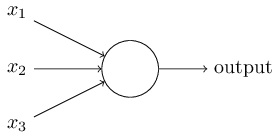
\includegraphics[scale = 0.7]{images/perceptron.png}
 \caption{\textit{Perceptron con 3 input ed un output}}
 \label{perceptron}
\end{figure}

l'output sarà determinato da:

\begin{center}
$\begin{cases}
 0 \text{ se } \sum_{i} x_{i}w_{i} \leq valore\text{ }di\text{ }soglia\\
 1 \text{ se } \sum_{i} x_{i}w_{i} > valore\text{ }di\text{ }soglia 
\end{cases} $
\end{center}

anche se è più comune trovare la scrittura:

\begin{center}
$\begin{cases}
 0 \text{ se } \sum_{i} x_{i}w_{i} + b \leq 0\\
 1 \text{ se } \sum_{i} x_{i}w_{i} + b > 0
\end{cases}$
\end{center}

dove $b$ è detto \textit{bias} del perceptron.
È attraverso \textit{pesi} e \textit{bias} che il perceptron può soppesare diverse prove e compiere decisioni.

Tuttavia se la rete contenesse perceptron, anche un piccolo cambiamento nei parametri interni potrebbe causare un cambiamento netto nel comportamento della rete [\cite{neural-net-nielsen}], per questo è preferibile utilizzare una \textit{funzione di attivazione} che rende continuo l'output di un nodo.
Un esempio di funzione di attivazione è la sigmoide definita come:

\begin{equation} \label{sigma}
 \sigma(z) = \frac{1}{1+e^{-z}} 
\end{equation}

e l'output di un nodo della rete diventa :

\begin{equation} \label{z}
  y = \sigma(\sum_{i}{x_{i}w_{i}} + b)
\end{equation}

risultato che è continuo e compreso tra zero ed uno.

Un altro tipo di funzione di attivazione è la \textit{Rectified Linear Units} o \textit{ReLU} e si presenta come:

\begin{equation}
 y(x) = max \{0,x\} 
\end{equation}

\begin{figure}[H]
 \centering
 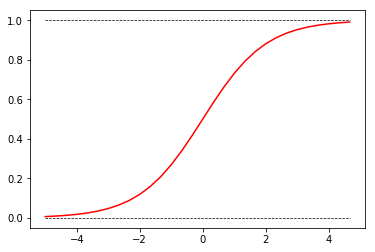
\includegraphics[scale = 0.5]{images/sigmoide.png}
 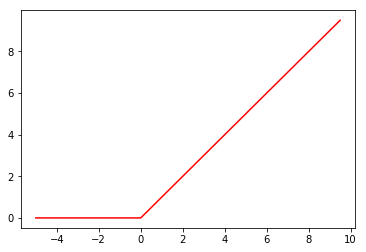
\includegraphics[scale = 0.5]{images/relu.png}
 \caption{\textit{confronto tra due funzioni di attivazione: a sinistra sigmoidale e a destra ReLU}}
 \label{sigmarelu}
\end{figure}

La scelta della migliore funzione di attivazione non è univoca e dipende dal problema che viene affrontato.

\subsection{Struttura \textit{fully connected}}

La struttura di una rete neurale \textit{fully connected} composta da molti \textit{layer} di neuroni è come quella mostrata in figura \ref{net}:

\begin{figure}[H]
 \centering
 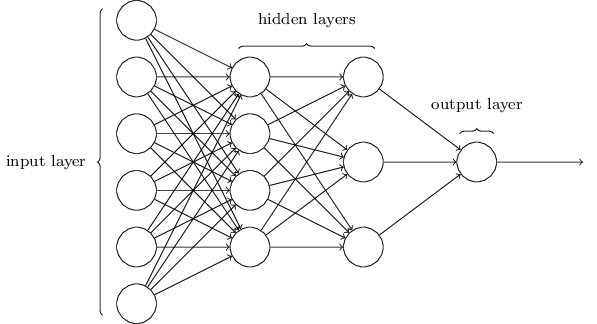
\includegraphics[scale = 0.5]{images/net.png}
 \caption{\textit{Esempio di rete neurale fully connected in cui viene mostrata la distinzione tra input layer, hidden layer e output layer}}
 \label{net}
\end{figure} 

In una rete come questa ad ogni collegamento è associato un peso e ad ogni nodo è associato un \textit{bias}: gli output dei \textit{neuroni} del \textit{layer} di input diventano a loro volta valori in ingresso del \textit{layer} successivo in un procedimento a catena fino all'ultimo \textit{layer}, che restituisce la risposta della rete. 
L'addestramento della rete consiste nel valutarne gli output in un determinato set di dati, chiamato \textit{training dataset}, confrontarli con i valori attesi, forniti dallo stesso \textit{dataset}, e modificare pesi e \textit{bias} in modo che la risposta si avvicini a ciò che ci si aspetta.


Da completare con algoritmo di BackPropagation???

\subsection{Evoluzione di una Rete Neurale}

\chapter{Metodologia}

\chapter{Risultati}

\chapter{Conclusioni}

\listoffigures

\nocite{*}
\addcontentsline{toc}{chapter}{Bibliografia}
\bibliographystyle{plainnat}
\bibliography{Bibliografia.bib}


\end{document}




